\section{Experiments}
\label{sec:experiments}
\vspace{-5pt}
\begin{table*}[h]
\scalebox{0.9}{
\centering
\begin{tabular}{llllllllllllllll|l}
\hline
\textbf{Scan} & 24   & 37   & 40   & 55   & 63   & 65   & 69   & 83   & 97   & 105  & 106  & 110  & 114  & 118  & 122  & Mean \\  
\hline
\hline
COLMAP \cite{schonberger2016structure} & \textbf{0.9} & 2.89 & 1.63 & 1.08 & 2.18 & 1.94 & 1.61 & 1.3  & 2.34 & 1.28 & 1.1  & 1.42 & 0.76 & 1.17 & 1.14 & 1.52 \\  
MVSNet \cite{yao2018mvsnet} & 1.05 & 2.52 & 1.71 & 1.04 & 1.45 & 1.52 & 0.88 & 1.29 & 1.38 & 1.05 & 0.91 & 0.66 & 0.61 & 1.08 & 1.16 & 1.22 \\  
CasMVSNet \cite{gu2020cascade} & 1.03 & 2.55 & 1.60 & 0.92 & 1.51 & 1.67 & 0.81 & 1.43 & 1.22 & 1.05 & 0.83 & 0.67 & 0.54 & 0.94 & 1.10 & 1.19 \\
\hline
VolSDF \cite{yariv2021volume} & 4.03 & 4.21 & 6.12 & 0.91 & 8.24 & 1.73 & 2.74 & 1.82 & 5.14 & 3.09 & 2.08 & 4.81 & 0.6  & 3.51 & 2.18 & 3.41 \\  
NeuS \cite{wang2021neus} & 4.57 & 4.49 & 3.97 & 4.32 & 4.63 & 1.95 & 4.68 & 3.83 & 4.15 & 2.5  & 1.52 & 6.47 & 1.26 & 5.57 & 6.11 & 4.00 \\  
3DGS \cite{kerbl20233d} & 3.01 & 2.71 & 2.11 & 1.96 & 4.07 & 3.35 & 2.48 & 3.4 & 2.74 & 2.91 & 3.31 & 3.29 & 1.73 & 2.73 & 2.51 & 2.82 \\  
2DGS \cite{huang20242d} & 3.12 & \textbf{2.12} & 2.18 & 1.41 & 3.74 & 2.39 & 2.18 & 2.84 & 2.87 & 1.93 & 3.71 & 3.88 & 1.07 & 3.02 & 2.01 & 2.56 \\  
MASt3R \cite{leroy2024grounding} & 1.62 & 3.06 & 3.74 & 1.50 & 1.75 & 2.70 & 1.65 & 1.82 & 2.64 & 1.80 & 1.52 & 1.43 & 1.20 & 1.52 & 1.37 & 1.95 \\  
% InstantSplat \cite{fan2024instantsplat} & 9.31 & 8.31 & 10.24 & 7.62 & 10.01 & 7.8 & 7.86 & 10.07 & 9.66 & 8.37 & 6.91 & 6.49 & 6.88 & 7.45 & 7.4 & 8.29 \\  
IBRNet-ft \cite{wang2021ibrnet} & 1.67 & 2.97 & 2.26 & 1.56 & 2.52 & 2.30 & 1.50 & 2.05 & 2.02 & 1.73 & 1.66 & 1.63 & 1.17 & 1.84 & 1.61 & 1.90 \\  
SparseNeuS-ft \cite{long2022sparseneus} & 1.29 & 2.27 & 1.57 & \underline{0.88} & 1.61 & 1.86 & 1.06 & 1.27 & 1.42 & 1.07 & 0.99 & 0.87 & \underline{0.54} & 1.15 & 1.18 & 1.27 \\  
\hline
IBRNet \cite{wang2021ibrnet} & 2.29 & 3.70 & 2.66 & 1.83 & 3.02 & 2.83 & 1.77 & 2.28 & 2.73 & 1.96 & 1.87 & 2.13 & 1.58 & 2.05 & 2.09 & 2.32 \\  
GeoNeRF \cite{johari2022geonerf} & 3.40 & 4.37 & 3.99 & 2.94 & 5.08 & 4.50 & 3.42 & 4.68 & 4.54 & 4.05 & 3.47 & 3.23 & 3.34 & 3.57 & 3.63 & 3.88 \\ 
SparseNeuS \cite{long2022sparseneus} & 1.68 & 3.06 & 2.25 & 1.1  & 2.37 & 2.18 & 1.28 & 1.47 & 1.8  & 1.23 & 1.19 & 1.17 & 0.75 & 1.56 & 1.55 & 1.64 \\ 
VolRecon \cite{ren2023volrecon} & 1.2  & 2.59 & 1.56 & 1.08 & 1.43 & 1.92 & 1.11 & 1.48 & 1.42 & 1.05 & 1.19 & 1.38 & 0.74 & 1.23 & 1.27 & 1.38 \\  
ReTR \cite{liang2024retr} & 1.05 & 2.31 & \underline{1.44} & 0.98 & 1.18 & 1.52 & 0.88 & 1.35 & 1.3  & 0.87 & 1.07 & 0.77 & 0.59 & 1.05 & 1.12 & 1.17 \\
GeoTransfer \cite{jena2024geotransfer} & 0.95 & \underline{2.23} & 1.45 & 0.94 & 1.26 & 1.67 & 0.81 & \underline{1.21} & 1.34 & 1.02 & \underline{0.84} & \underline{0.6} & 0.58 & 0.94 & \underline{1.02} & 1.12 \\ 
% UfoRecon \cite{ren2023volrecon} & 0.76 & 2.05 & 1.31 & 0.82 & 1.12 & 1.18 & 0.74 & 1.17 & 1.11 & 0.71 & 0.88 & 0.58 & 0.54 & 0.86 & 0.99 &  0.99 \\
UfoRecon$^{\ast}$\footnotemark[1] \cite{ren2023volrecon} & \underline{0.91}  & 2.32 & \textbf{1.41} & 0.89 & \underline{1.17} & \textbf{1.21} & \underline{0.74} & 1.24 & \textbf{1.18} & \textbf{0.83} & \textbf{0.77} & 0.64 & 0.56 & \underline{0.89} & \underline{1.02} & \underline{1.05} \\  
\hline
Ours & 0.97 & 2.28 & 1.5 & \textbf{0.85} & \textbf{1.14} & \underline{1.26} & \textbf{0.73} & \textbf{1.19} & \underline{1.2} & \underline{0.86} & \textbf{0.77} & \textbf{0.58} & \textbf{0.48} & \textbf{0.84} & \textbf{0.95} & \textbf{1.04} \\  
\hline
\end{tabular}
}
\caption{Quantitative comparison on the DTU dataset \cite{aanaes2016large}. Best and second best methods are \textbf{emboldened} and \underline{underlined} respectively. UfoRecon$^{\ast}$ \cite{ren2023volrecon} refers to the results generated with pretrained model provided in their code.\\ (Inference time: Ours 0.8s, UfoRecon\cite{ren2023volrecon} 66s)} \label{tab:table1}
\vspace{-7pt}
\end{table*}

In this section, we showcase the performance of our proposed approach. Firstly, we offer an overview of our experimental configurations, implementation specifics, datasets, and baseline methods. Secondly, we present both quantitative and qualitative comparisons on three commonly used multi-view datasets, namely DTU \cite{aanaes2016large}, BlendedMVS \cite{yao2020blendedmvs} and Tanks and Temples \cite{knapitsch2017tanks}. Finally, we perform ablation studies to evaluate the impact of the components of our proposed method.
\vspace{-15pt}
\paragraph{Datasets}
In line with prior research \cite{long2022sparseneus, ren2023volrecon, liang2024retr, na2024uforecon}, we employ the DTU dataset \cite{aanaes2016large} for the training phase. The DTU dataset \cite{aanaes2016large} is characterized by indoor multi-view stereo data, featuring ground truth point clouds from 124 distinct scenes and under 7 different lighting conditions. Throughout our experiments, we utilize the same set of 15 scenes as \cite{long2022sparseneus, ren2023volrecon, liang2024retr, jena2024geotransfer, na2024uforecon} for testing purposes, reserving the remaining scenes for training. Concerning the BlendedMVS dataset \cite{yao2020blendedmvs}, we opt for the same scenes as used in SparseNeuS \cite{long2022sparseneus}, with some additional ones chosen randomly. For each scene in either DTU \cite{aanaes2016large} or BMVS \cite{yao2020blendedmvs}, we use the same $3$ sparse input views following SparseNeuS \cite{long2022sparseneus}. To ensure impartial evaluation on DTU \cite{aanaes2016large}, we use the foreground masks from IDR \cite{yariv2020multiview} to mask the reconstructed meshes and evaluate how well our approach performs on the test set, consistent with prior research \cite{long2022sparseneus, ren2023volrecon, liang2024retr, jena2024geotransfer, na2024uforecon}. Additionally, to assess the generalization capability of our proposed framework, we qualitatively compare our method on the BlendedMVS dataset \cite{yao2020blendedmvs} and provide some additional examples om the Tanks and Temples dataset \cite{knapitsch2017tanks} without any fine-tuning. For our novel-view synthesis experiments, we follow the same split of testing images within a scene as well as the same testing scenes as in MVSGaussian \cite{liu2024fast}. We also include some additional reconstruction and novel view synthesis qualitative comparisons in the supplementary material, including some video examples.

% \todo{say somewhere in results what we show in supp material}

\vspace{-15pt}
\paragraph{Baselines}
In order to showcase the efficacy of our method, we conducted comparisons with a) SparseNeus \cite{long2022sparseneus}, VolRecon \cite{ren2023volrecon}, ReTR \cite{liang2024retr}, GeoTransfer \cite{jena2024geotransfer} and UfoRecon \cite{na2024uforecon}, the leading generalizable neural surface reconstruction approaches; b) Generalizable neural/$3$DGS rendering methods PixelNeRF \cite{yu2021pixelnerf}, IBRNet \cite{wang2021ibrnet}, MVSNeRF \cite{chen2021mvsnerf}, GeoNeRF \cite{johari2022geonerf}, and MVSGaussian \cite{liu2024fast}; c) Neural implicit reconstruction methods VolSDF \cite{yariv2021volume}, NeuS \cite{wang2021neus} and Gaussian Splatting based methods 3D Gaussian Splatting \cite{kerbl20233d} and 2D Gaussian Splatting \cite{huang20242d} that necessitate scene-specific training; and finally, d) Well-established multi-view stereo (MVS) methods Colmap \cite{schonberger2016structure}, MVSNet \cite{yao2018mvsnet}, and CasMVSNet \cite{gu2020cascade} as well as MASt3R \cite{leroy2024grounding}. 
\vspace{-15pt}
\paragraph{Implementation details}
Our model is implemented using PyTorch \cite{paszke2019pytorch}. During training, we utilize an image resolution of $640 \times 512$, with $N$ (the number of source images) set to $3$. Network architecture follows mostly \cite{liu2024fast}. Training extends over $300$k steps using the Adam optimizer \cite{kingma2014adam} on a single RTX A$6000$ GPU, with an initial learning rate of $5 \times 10^{-4}$. To extract meshes from the reconstructed $2$D splats, we render depth maps of the training views. We then utilize truncated signed distance function (TSDF) fusion to combine the reconstructed depth maps. During TSDF fusion, we set the voxel size to $1.5$ following \cite{long2022sparseneus, ren2023volrecon, liang2024retr, jena2024geotransfer, na2024uforecon}.

\subsection{Sparse View Reconstruction on DTU}
\vspace{-5pt}
We conduct surface reconstruction with sparse views (only $3$ views) on the DTU dataset \cite{aanaes2016large} and assess the predicted surface by comparing it to the ground-truth point clouds using the chamfer distance metric. To facilitate a fair comparison, we followed the evaluation process employed in \cite{long2022sparseneus, ren2023volrecon, liang2024retr, jena2024geotransfer, na2024uforecon} and adhered to the same testing split as described in them. As indicated in Tab. \ref{tab:table1}, we offer superior results compared to neural implicit \cite{yariv2021volume, wang2021neus} and Gaussian Splatting based \cite{kerbl20233d, huang20242d} methods that use scene-specific training, but struggle in sparse input-view setup to lack of prior knowledge. We clearly outperform MASt3R \cite{leroy2024grounding} as well, where the mesh reconstructions for MASt3R have been obtained by performing TSDF fusion (with the same voxel size of $1.5$) on the depth maps inferred by MASt3R. Additionally, our method (only DTU trained) surpasses almost all the generalizable implicit methods \cite{long2022sparseneus, ren2023volrecon, liang2024retr} by a good margin, \ie by $36.58\%$, $32.69\%$ and $12.5\%$ respectively. Furthermore, our approach exhibits superior performance compared to well-known multi-view stereo (MVS) methods like Colmap \cite{schonberger2016structure}, MVSNet \cite{yao2018mvsnet} and CasMVSNet \cite{gu2020cascade}. Our approach also demonstrates superior performance in comparison to GeoTransfer \cite{jena2024geotransfer} (by $7.14\%$) and narrowly outperforms UfoRecon \cite{na2024uforecon}, which are the latest state-of-the-art generalizable neural implicit reconstruction methods. Here, we report results for UfoRecon \cite{na2024uforecon} by averaging chamfer metrics over multiple runs using their code and pretrained model\footnotemark[1]\footnotetext[1]{\href{https://github.com/Youngju-Na/UFORecon}{https://github.com/Youngju-Na/UFORecon}}. Despite our best efforts, we could not reproduce the chamfer metrics originally reported in their paper. Additionally, we present qualitative results of sparse view reconstruction in Fig.\ref{fig:DTU}, showcasing that our reconstructed geometry features more expressive and detailed surfaces compared to the current state-of-the-art methods.

%which represent the ground truth surfaces more accurately when compared to the current state-of-the-art methods.

\begin{figure*}
    \centering
    %\includegraphics[width=1.0\linewidth]{figs/DTU_reconstructions.png}
    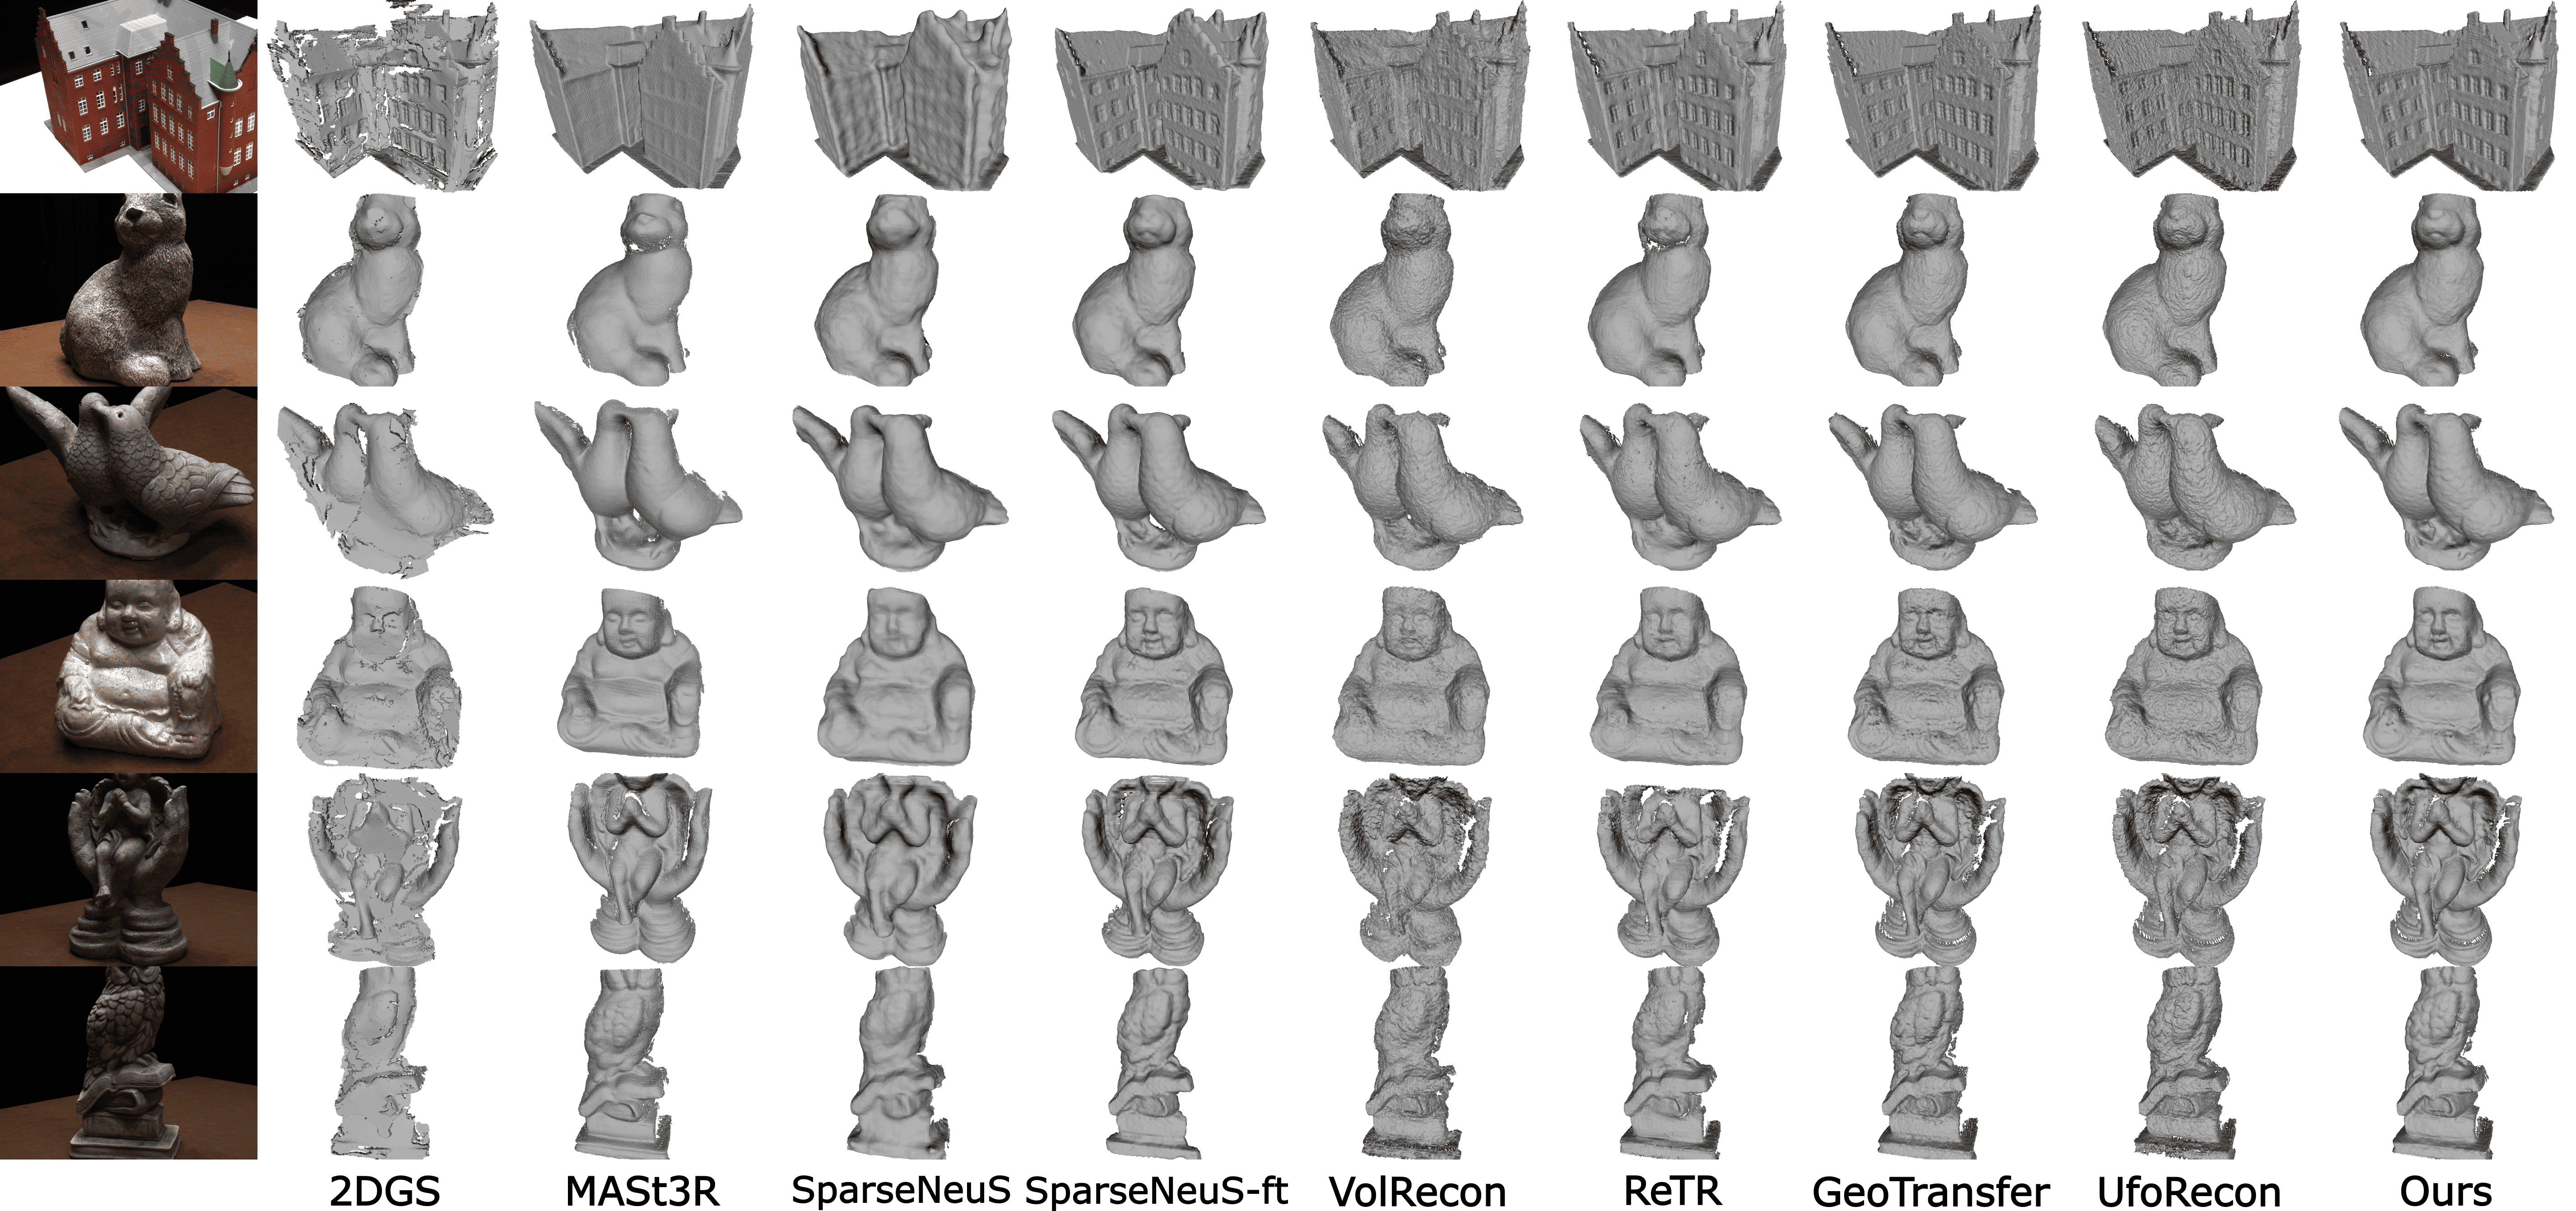
\includegraphics[width=1.0\linewidth]{figs/dtu.png}
    \vspace{-15pt}
    \caption{Qualitative comparison of reconstructions from 3 input views in datatset DTU. (Inference time: Ours 0.8s, UfoRecon\cite{ren2023volrecon} 66s).}
    \vspace{-8pt}
    \label{fig:DTU}
\end{figure*}

\subsection{Generalization on BlendedMVS and Tanks and Temples} 
\vspace{-5pt}
To demonstrate the generalization prowess of our proposed approach, we perform additional evaluations on the BlendedMVS dataset \cite{yao2020blendedmvs} without resorting to any fine-tuning. The high-fidelity reconstructions of scenes and objects, as illustrated in Fig. \ref{fig:BMVS}, affirms the efficacy of our method in terms of its generalization capabilities. Our method is able to obtain more detailed surfaces in comparison to Colmap \cite{schonberger2016structure}, SparseNeuS \cite{long2022sparseneus}, GeoTransfer \cite{jena2024geotransfer} as well as the recent SOTA UfoRecon \cite{na2024uforecon}.

\begin{figure}
    \centering
    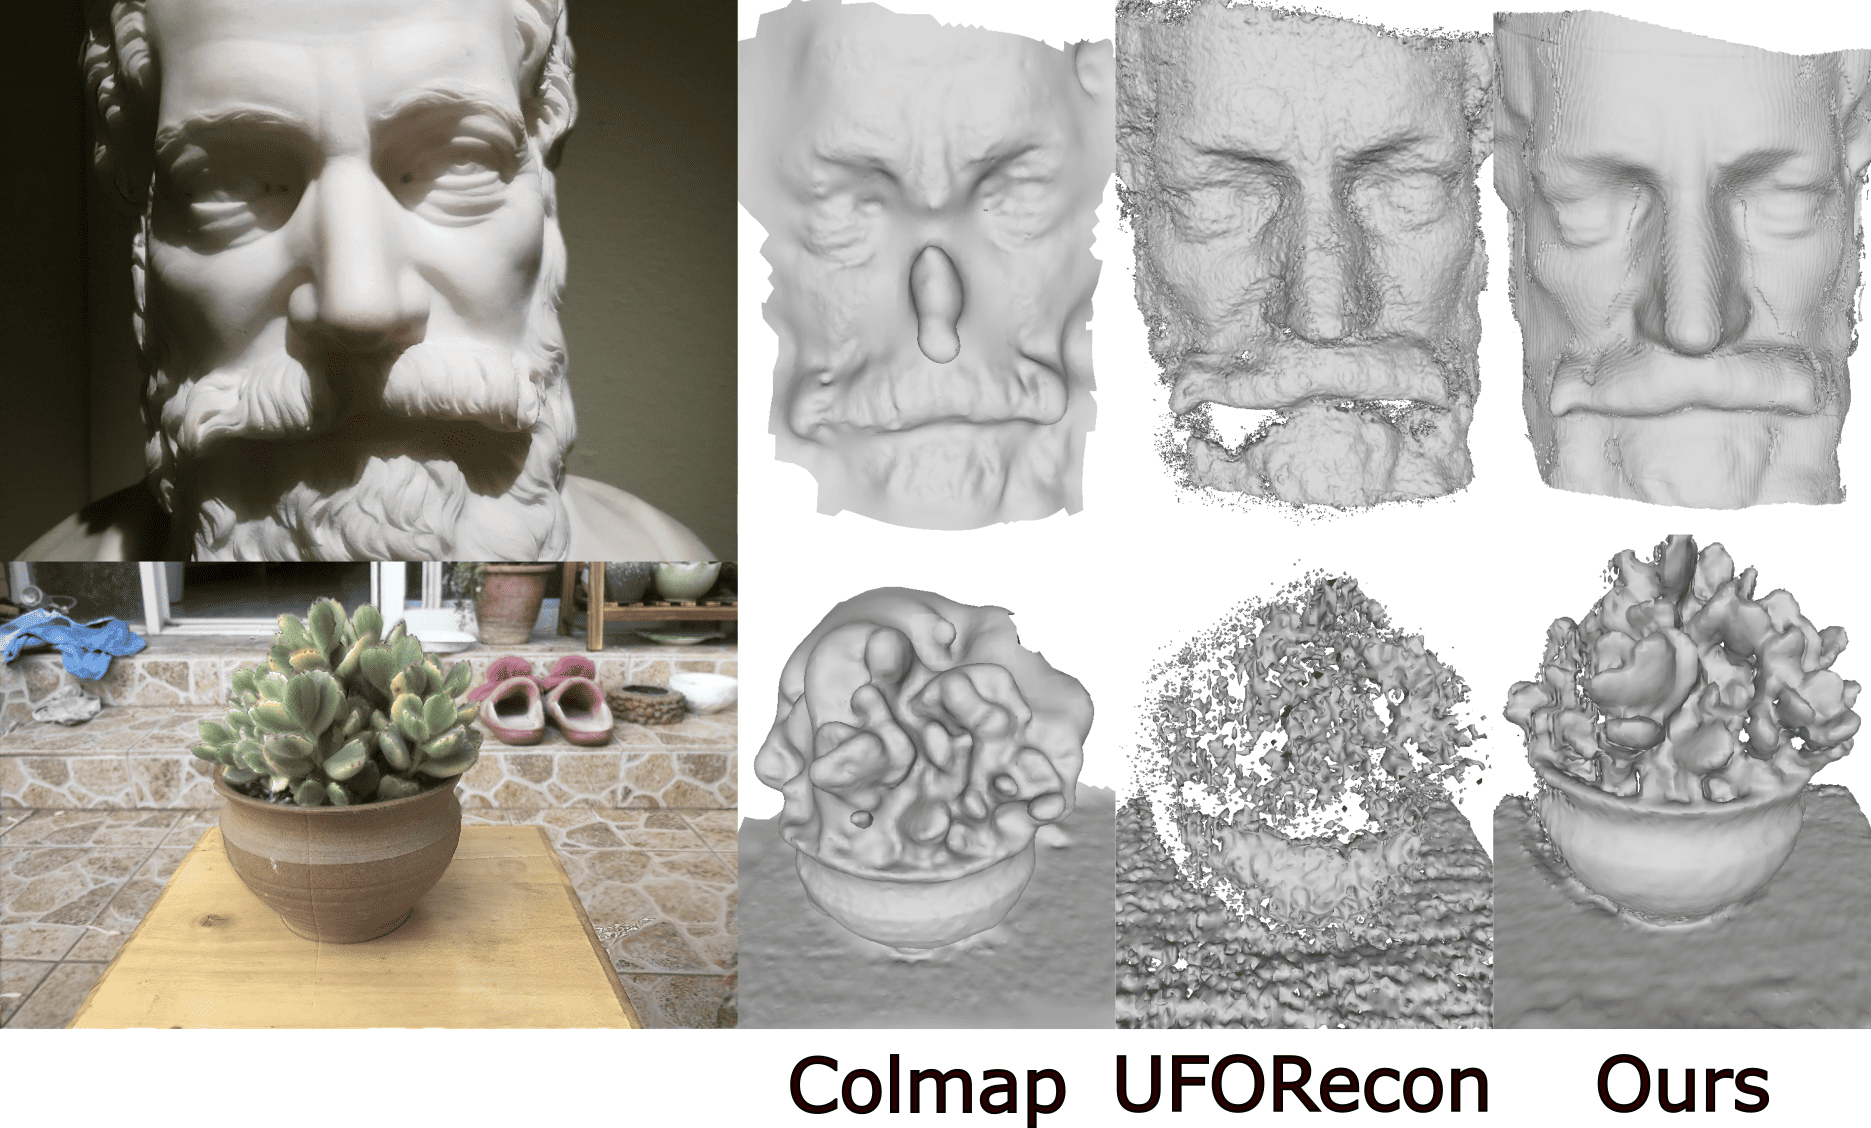
\includegraphics[width=1.0\linewidth]{figs/bmvs1.png}
    \\
    \vspace{5pt}
    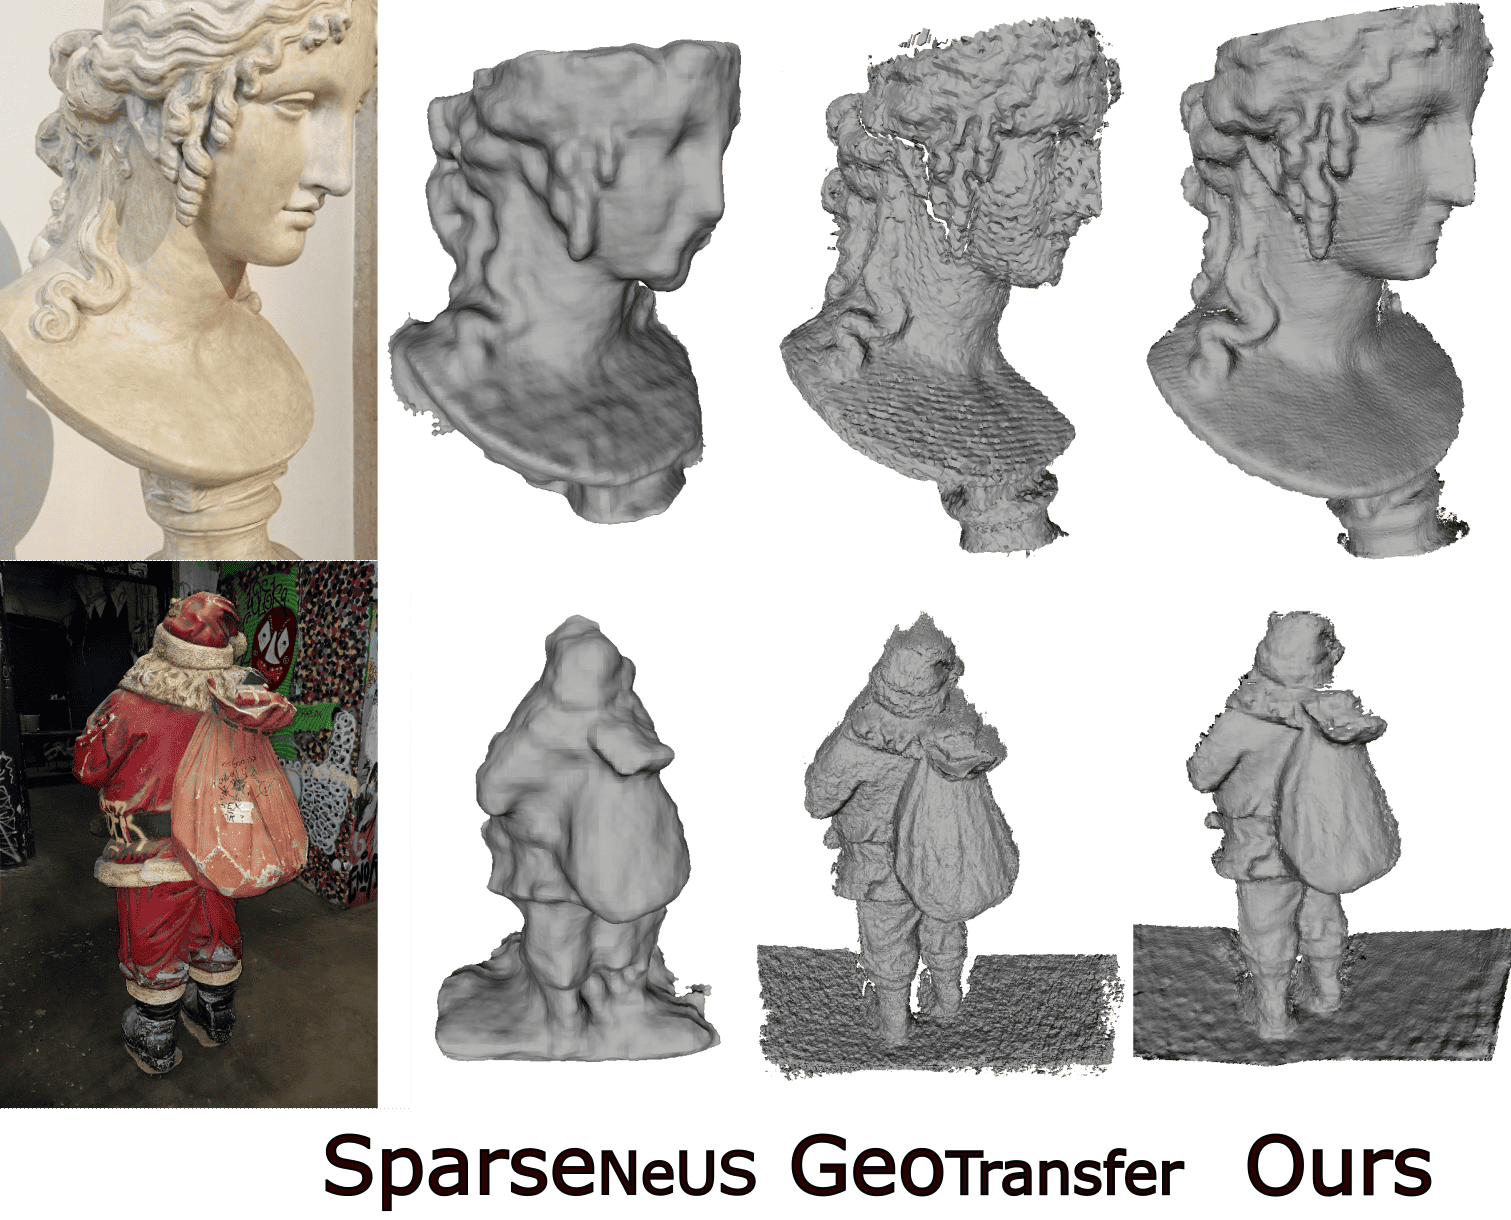
\includegraphics[width=0.88\linewidth]{figs/bmvs2.png}
    %\vspace{-10pt}
    \caption{Qualitative comparison of reconstructions from 3 input views in datatset BMVS. Note that we reconstruct detailed surfaces with our method without any fine-tuning.}
    \vspace{-10pt}
    \label{fig:BMVS}
\end{figure}

%\subsection{Generalization on Tanks and Temples}
As shown in Fig. \ref{fig:TNT}, we further emphasize the generalization capabilities of our method by providing reconstruction examples on scenes of the Tanks and Temples dataset.
% \begin{figure*}[t]
%     \centering
%     \setlength{\tabcolsep}{1pt} % Adjust space between images if needed
%     \begin{tabular}{@{}cccc@{}}
%         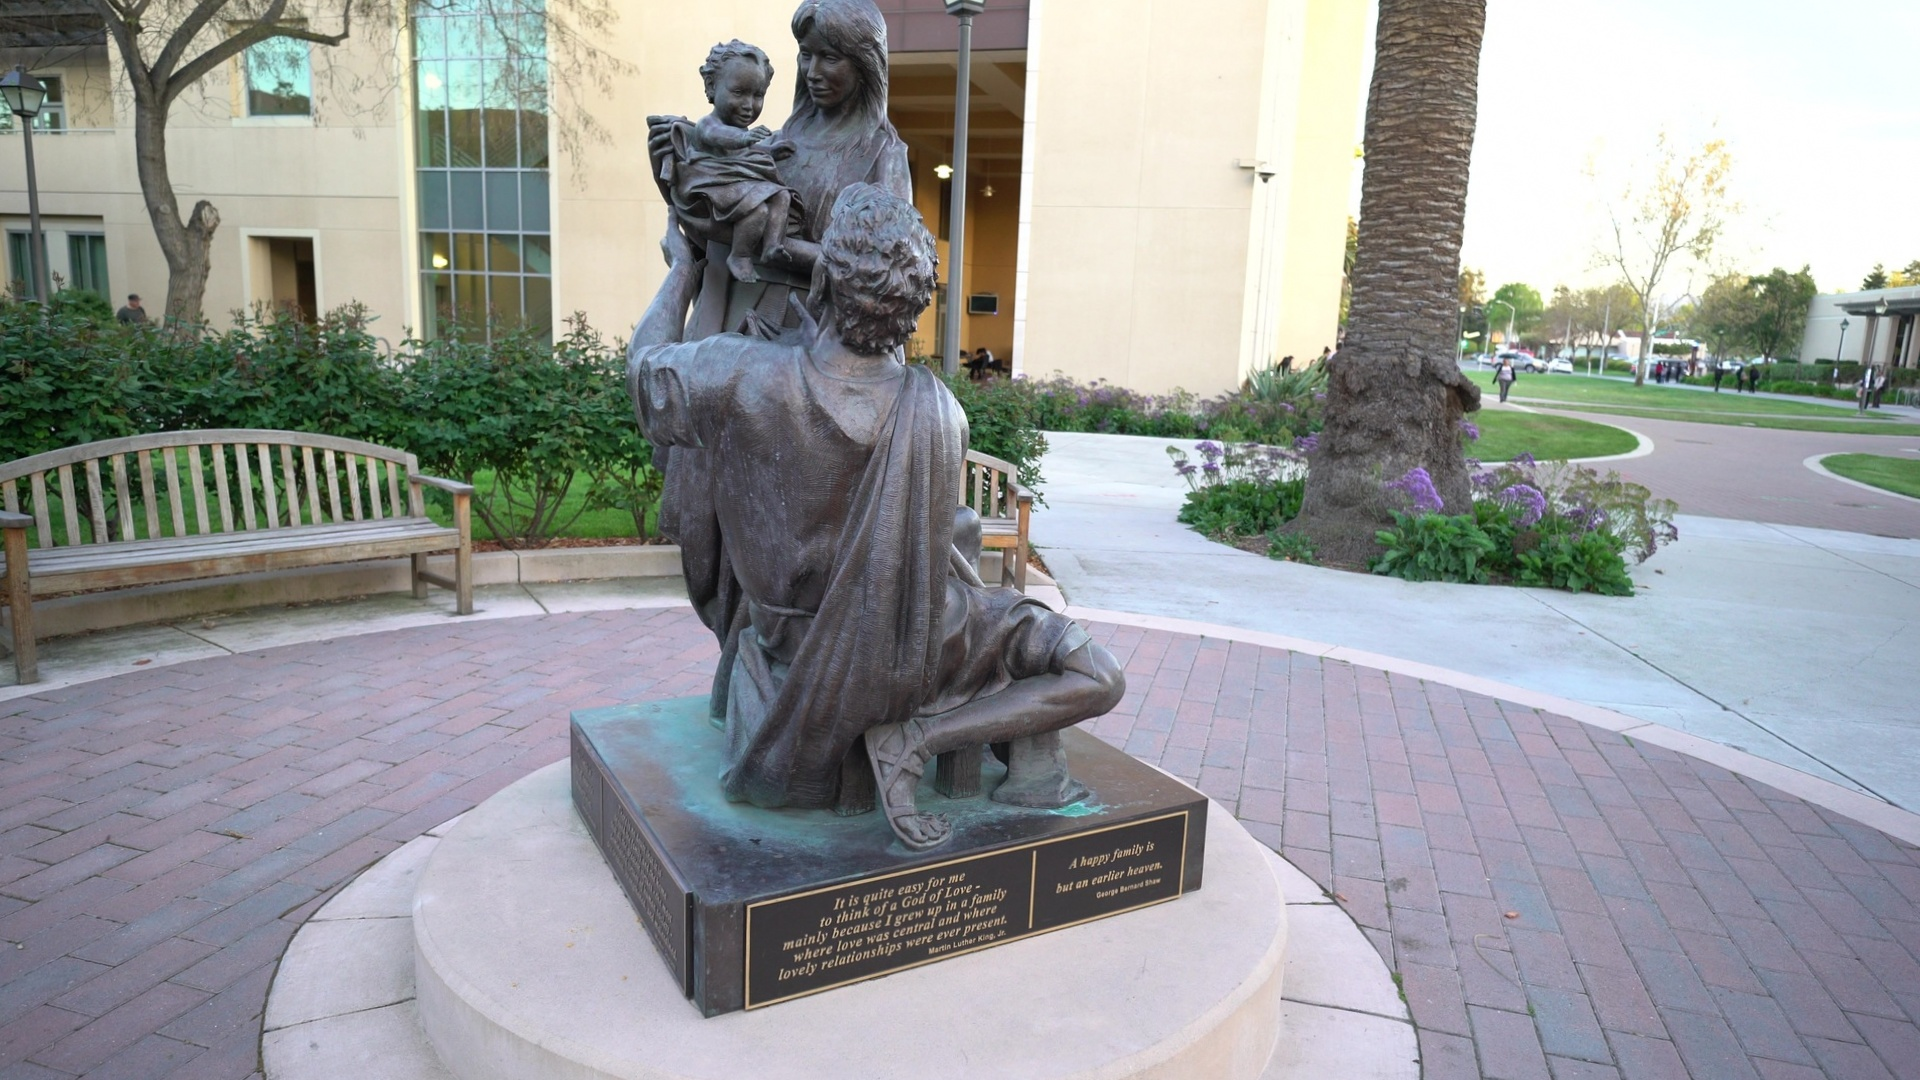
\includegraphics[width=0.24\linewidth]{figs/TNT/00000012.jpg} & 
%         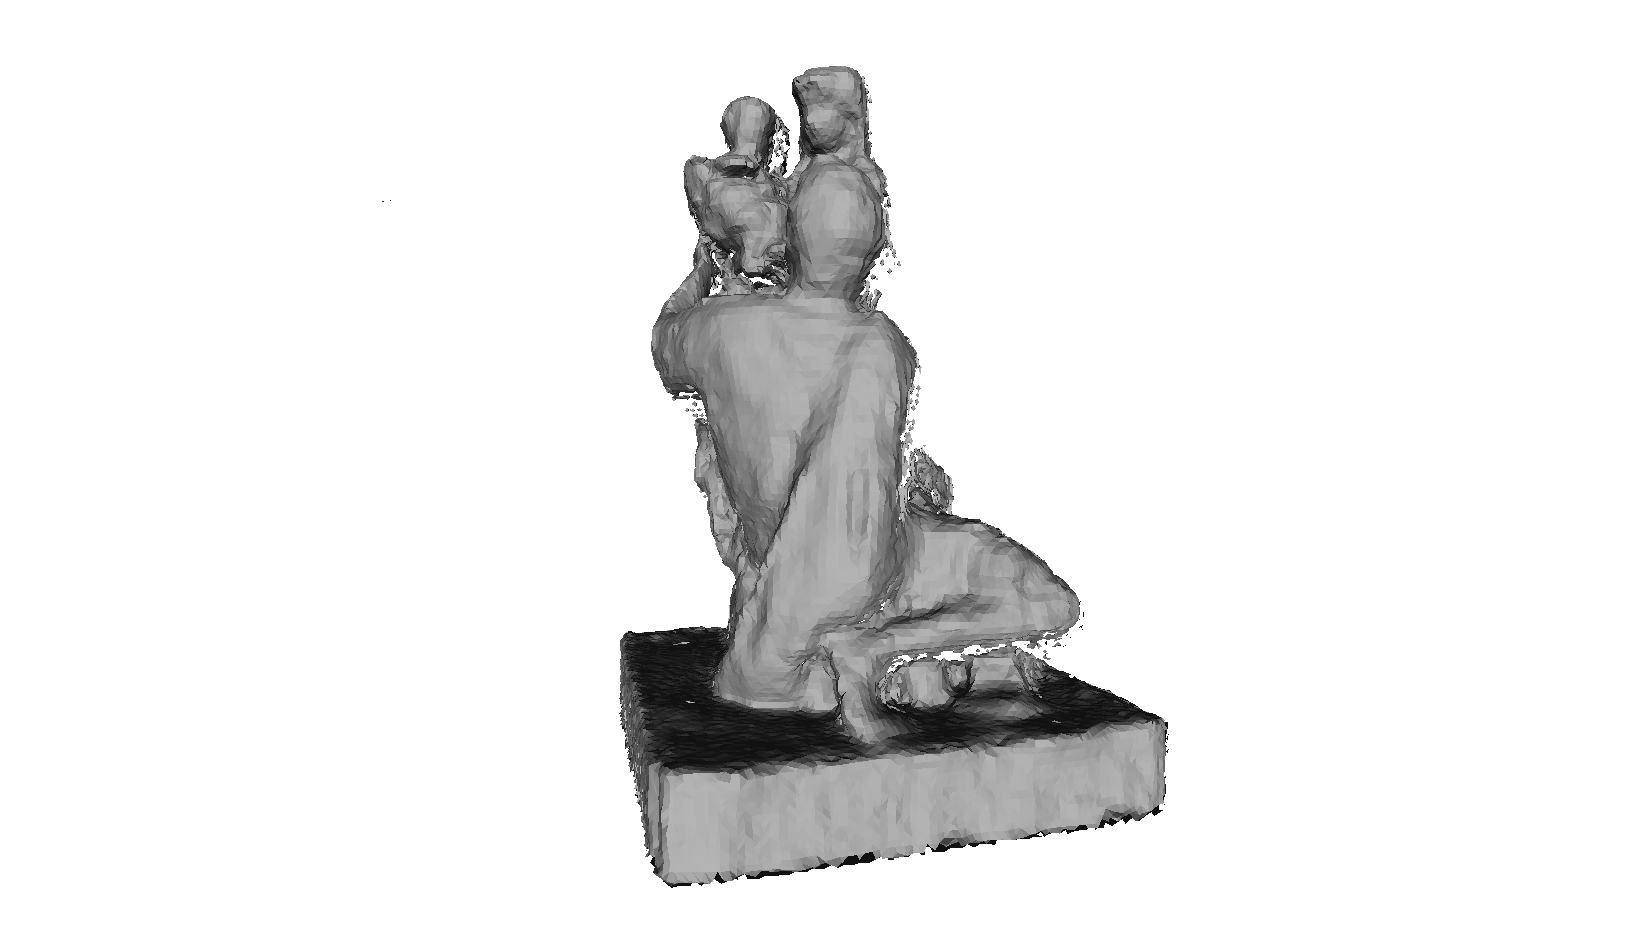
\includegraphics[width=0.24\linewidth]{figs/TNT/snapshot01.png} & 
%         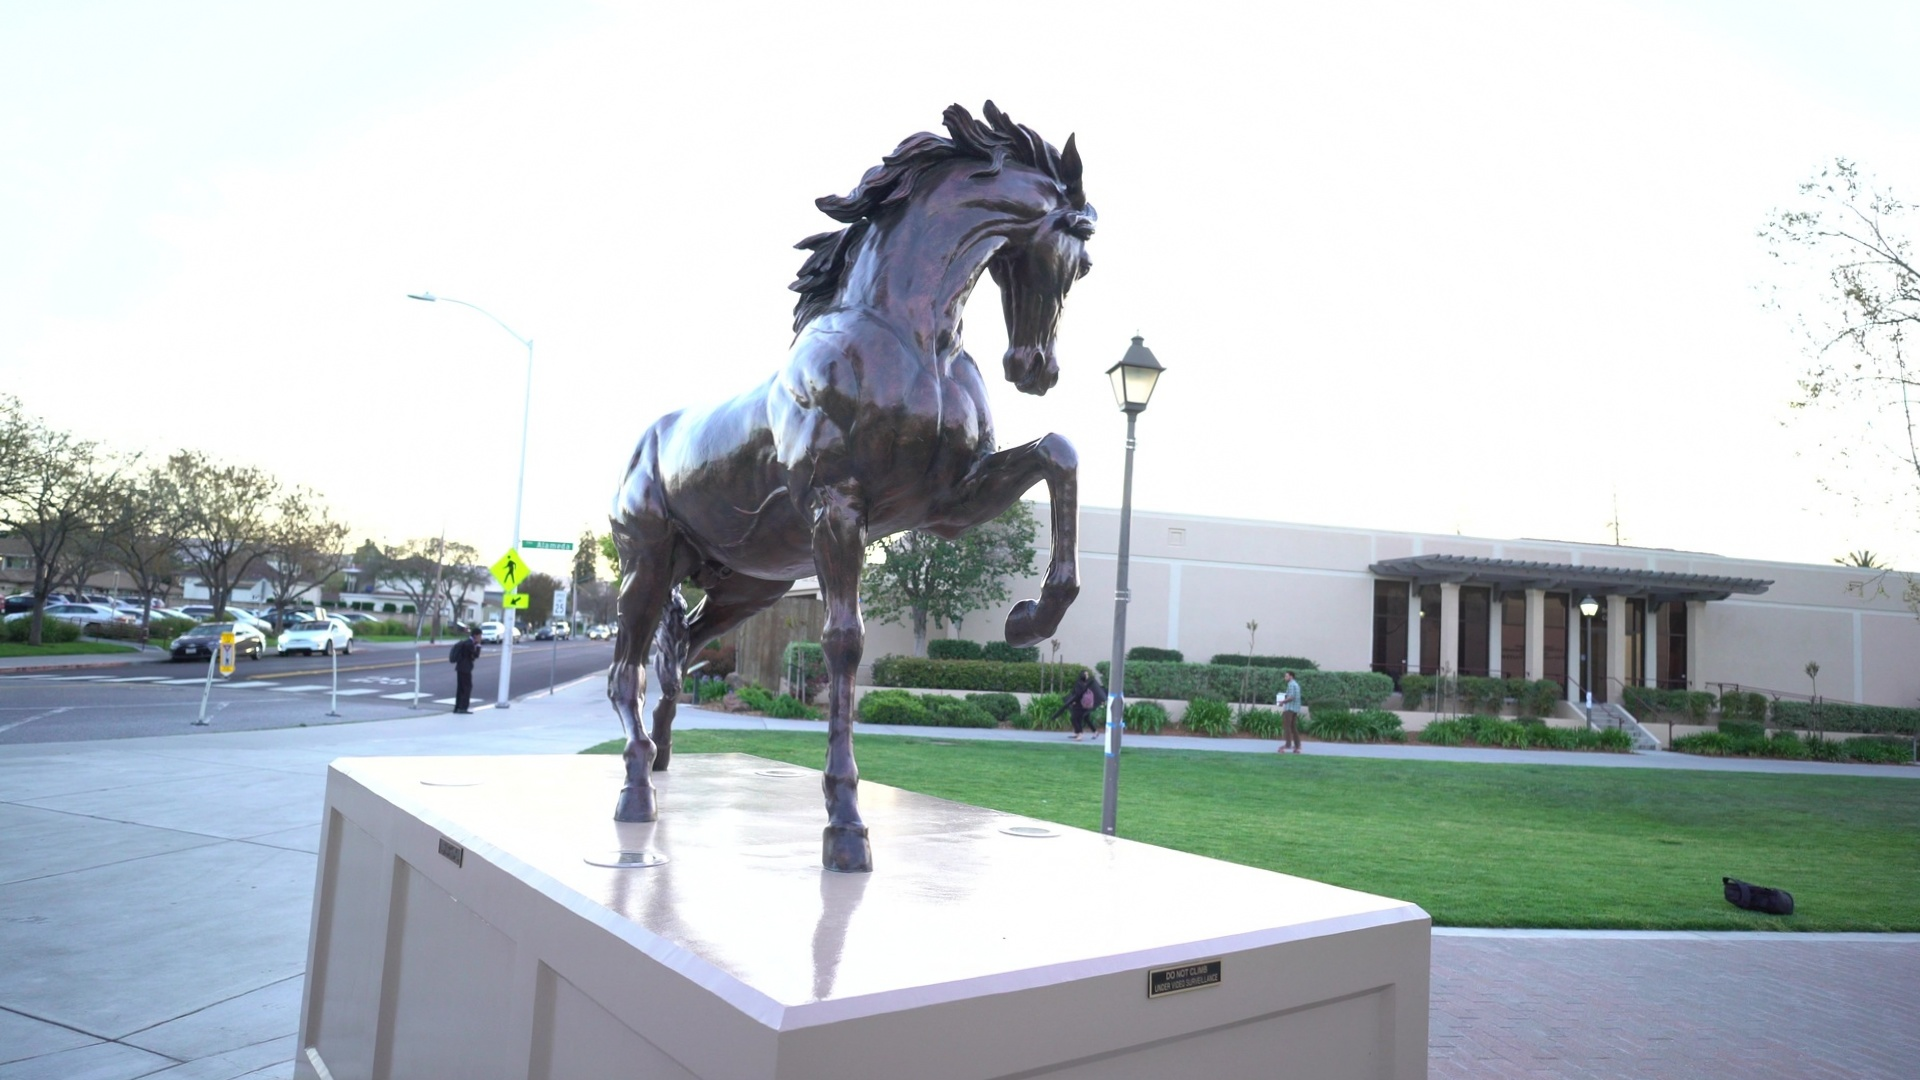
\includegraphics[width=0.24\linewidth]{figs/TNT/00000036.jpg} & 
%         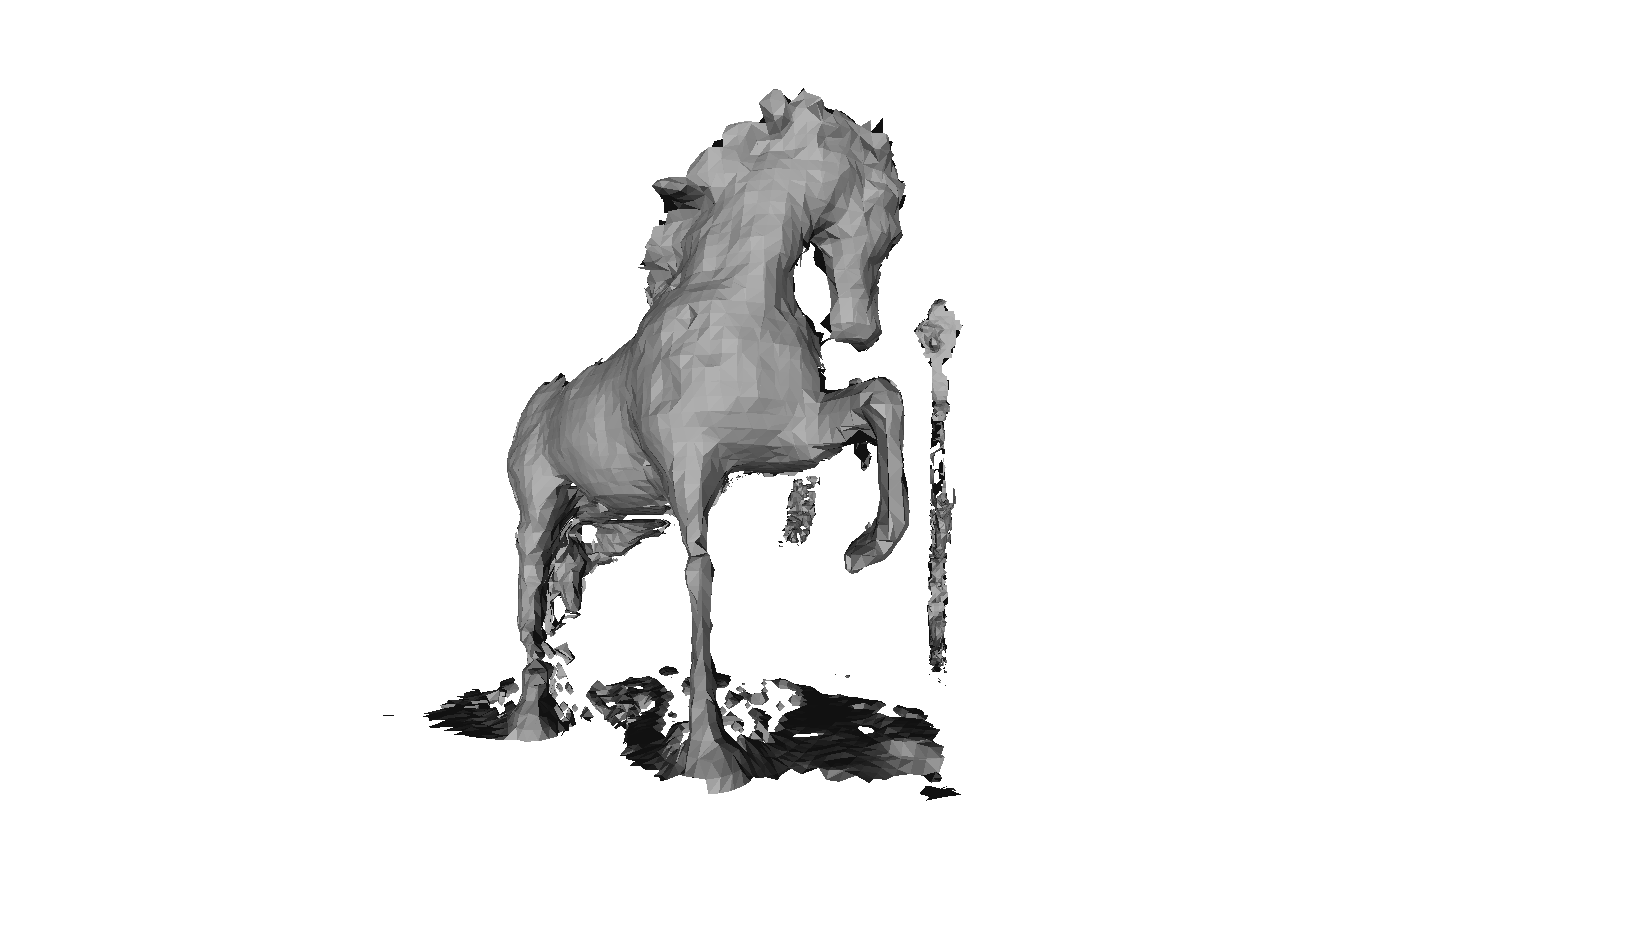
\includegraphics[width=0.24\linewidth]{figs/TNT/snapshot03.png} \\
%         GT & Ours & GT & Ours \\
%     \end{tabular}
%     \caption{Qualitative comparison of reconstructions from 3 input views in datatset Tanks and Temples without any fine-tuning.}
%     \label{fig:TNT}
% \end{figure*}

\begin{figure}
    \centering
    \includegraphics[width=1.0\linewidth]
    %{figs/TNT_Reconstructions.png}
    {figs/TNT/3.png}
    \caption{Qualitative results of reconstructions from 3 input views in datatset Tanks and Temples using our method without any fine-tuning. Notice that these are very challenging outdoor cases.}
    \vspace{-10pt}
    \label{fig:TNT}
\end{figure}


%\vspace{-5pt}

\begin{figure*}[t!]
    \centering
    \setlength{\tabcolsep}{1pt}
    \begin{minipage}{\linewidth}
    \centering
    \begin{tabular}{@{}cccccc@{}}
        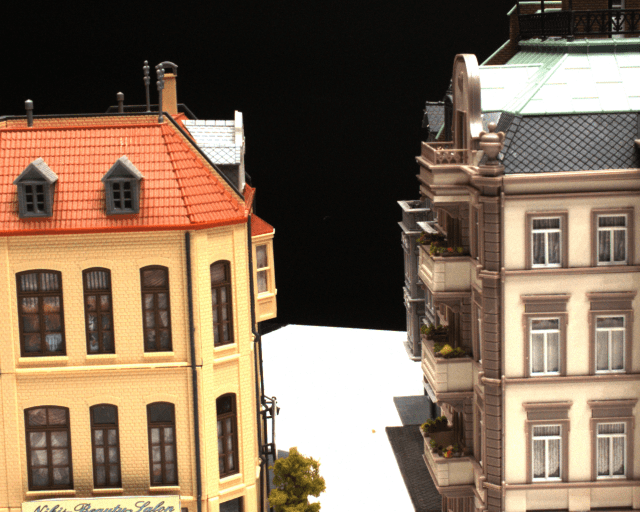
\includegraphics[width=0.162\linewidth]{figs/NVS/scan21_44_0_gt.png} & 
        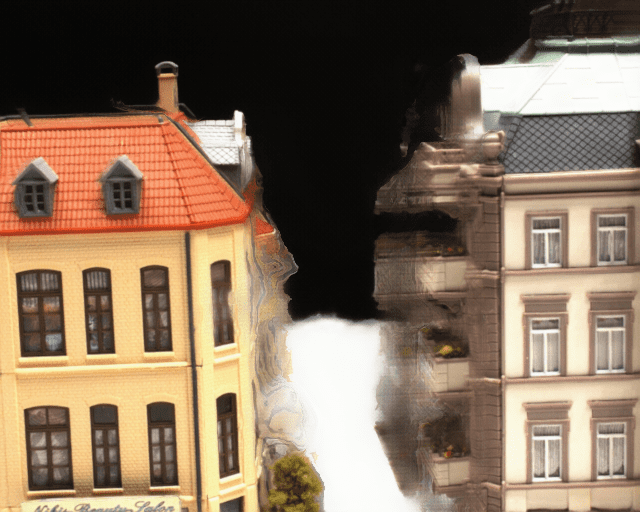
\includegraphics[width=0.162\linewidth]{figs/NVS/scan21_44_0_pred_mvsgs.png} & 
        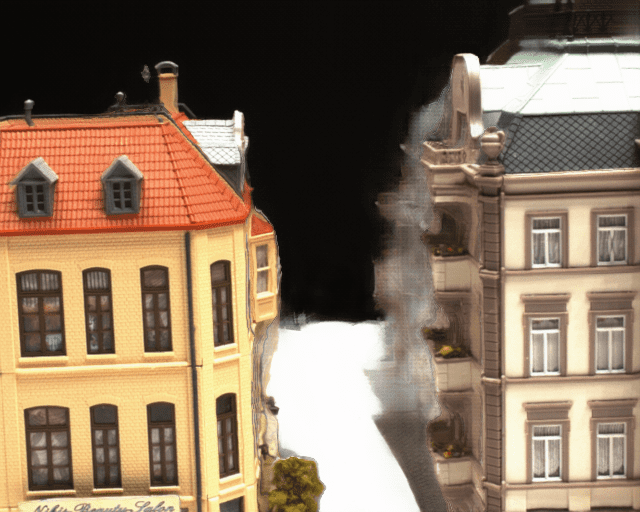
\includegraphics[width=0.162\linewidth]{figs/NVS/scan21_44_0_pred_ours.png} &
        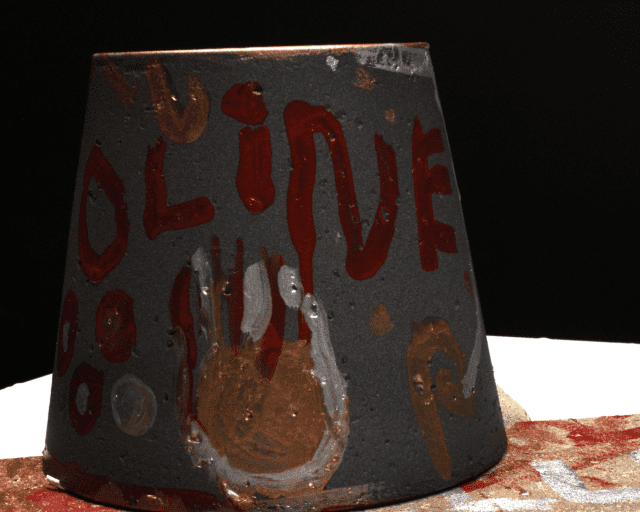
\includegraphics[width=0.162\linewidth]{figs/NVS/scan1_44_0_gt.png} & 
        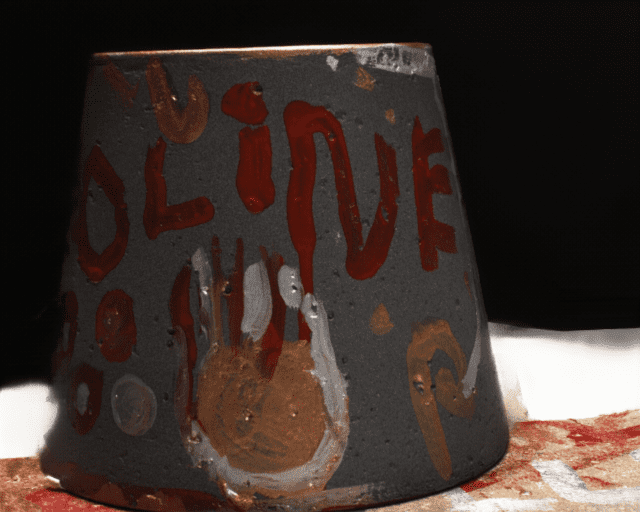
\includegraphics[width=0.162\linewidth]{figs/NVS/scan1_44_0_pred_mvsgs.png} & 
        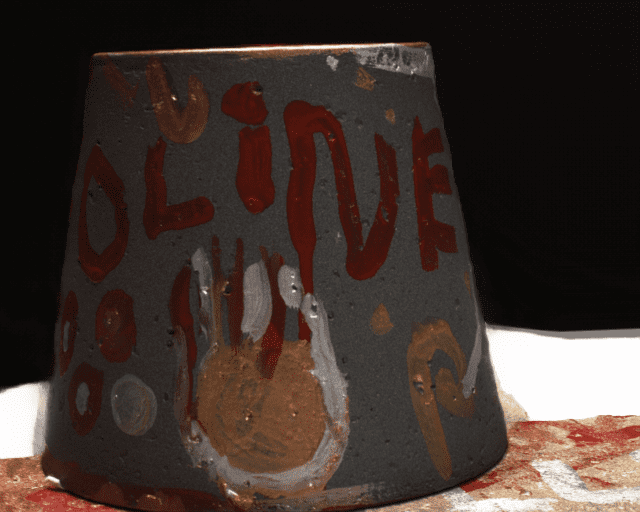
\includegraphics[width=0.162\linewidth]{figs/NVS/scan1_44_0_pred_ours.png} \\
        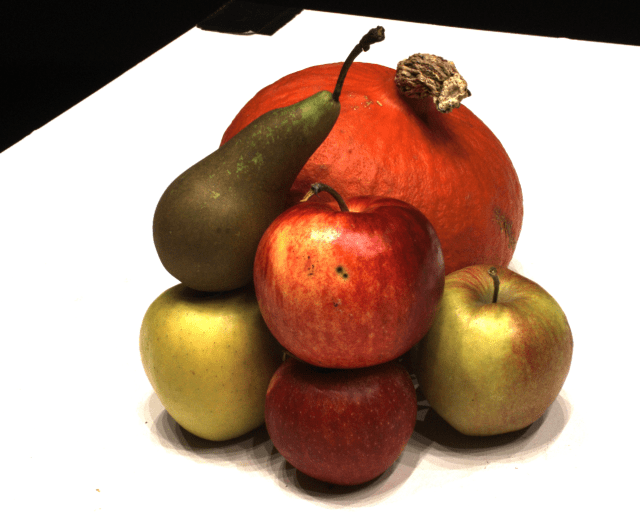
\includegraphics[width=0.162\linewidth]{figs/NVS/scan63_24_0_gt.png} & 
        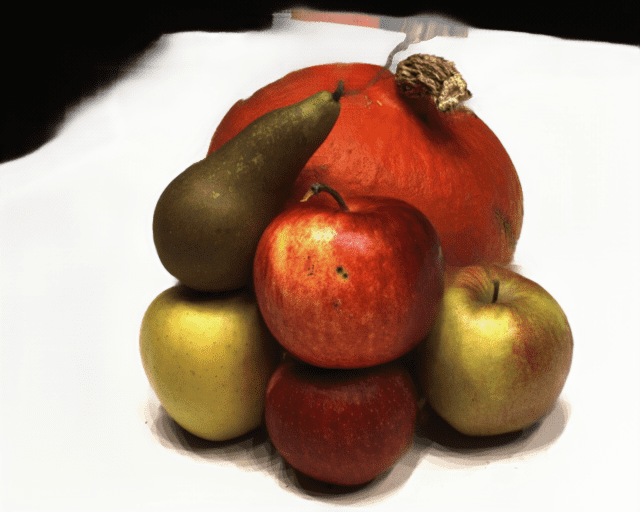
\includegraphics[width=0.162\linewidth]{figs/NVS/scan63_24_0_pred_mvsgs.png} & 
        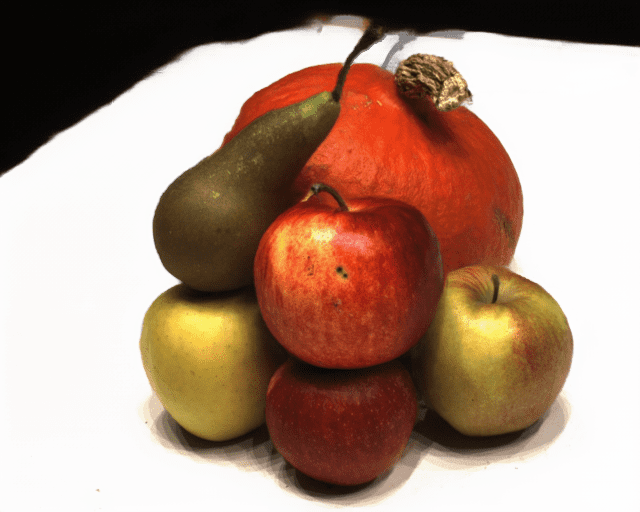
\includegraphics[width=0.162\linewidth]{figs/NVS/scan63_24_0_pred_ours.png} & 
        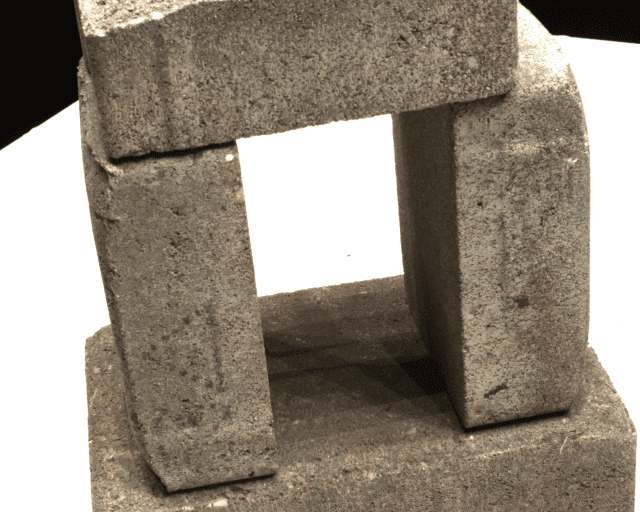
\includegraphics[width=0.162\linewidth]{figs/NVS/scan40_24_0_gt.png} & 
        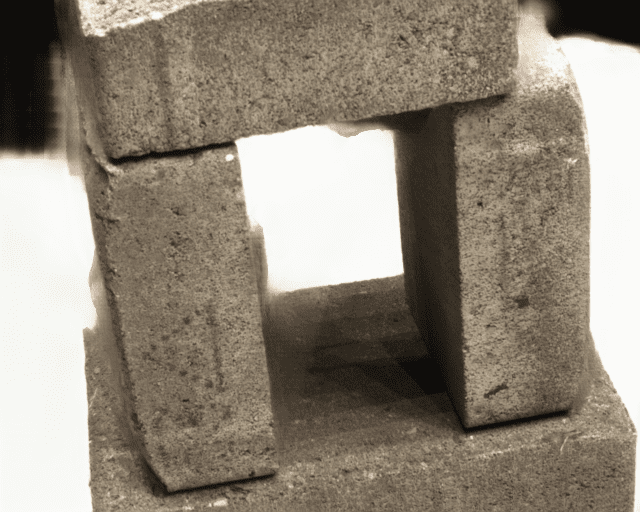
\includegraphics[width=0.162\linewidth]{figs/NVS/scan40_24_0_pred_mvsgs.png} & 
        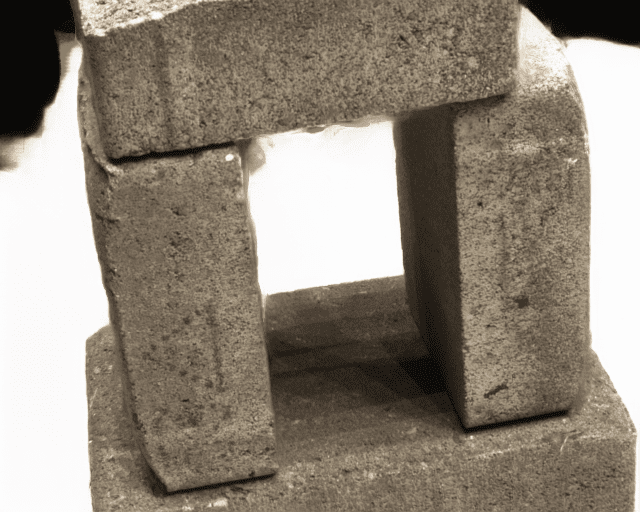
\includegraphics[width=0.162\linewidth]{figs/NVS/scan40_24_0_pred_ours.png} \\
        GT & MVSGaussian \cite{liu2024fast} & Ours & GT & MVSGaussian \cite{liu2024fast} & Ours \\
    \end{tabular}
    \end{minipage}
    \caption{Novel-View synthesis qualitative evalutation on DTU \cite{aanaes2016large} using $3$ source images. We outperform SOTA MVSGaussian \cite{liu2024fast} and exhibit sharper view synthesis results in regions with low input view overlap}
    \label{fig:nvs_grid}
\end{figure*}



\subsection{Novel-view synthesis on DTU}
\vspace{-5pt}
%Since MVSGaussian \cite{liu2024fast} is the recent state-of-the-art method for sparse novel-view synthesis, it is reasonable to assume that we also inherit its novel-view synthesis performance since we train our method by transferring its features. To validate this, 
We evaluate novel-view synthesis results on the DTU \cite{aanaes2016large} dataset. We compare our method against 
MVSGaussian \cite{liu2024fast} qualitatively (as shown in Fig. \ref{fig:nvs_grid}) as well as other
recent methods quantitatively on the mean PSNR, SSIM and LPIPS metrics over all scenes by following the same data split for training and testing as them. We use $3$ input source images for all the methods concerned. Our results can be summarized in Tab.\ref{tab:dtu_nv}.
\begin{table}[t]
\centering
\setlength{\tabcolsep}{5pt}
\resizebox{0.8\linewidth}{!}{
\begin{tabular}{@{}lccc@{}}
\toprule
Method & PSNR $\uparrow$ & SSIM $\uparrow$ & LPIPS $\downarrow$ \\
\midrule
PixelNeRF~\cite{yu2021pixelnerf} & 19.31 & 0.789 & 0.382 \\
IBRNet~\cite{wang2021ibrnet} & 26.04 & 0.917 & 0.191 \\ 
MVSNeRF~\cite{chen2021mvsnerf}  & 26.63 & 0.931 & 0.168 \\
ENeRF~\cite{lin2022efficient}  & 27.61 & 0.957 & 0.089 \\
MatchNeRF~\cite{chen2023explicit} & 26.91 & 0.934 & 0.159 \\
MVSGaussian~\cite{liu2024fast} & \underline{28.21} & \textbf{0.963} & \underline{0.076} \\
Ours & \textbf{28.33} & \underline{0.938} & \textbf{0.073} \\
\bottomrule
\end{tabular}
}
\caption{Quantitative results of NVS generalization on the DTU test set. The best result is \textbf{bold}, and the second-best is \underline{underlined}.}
\label{tab:dtu_nv}
\end{table}
This experiment illustrates that robust features of the $3$D foundation model MASt3R aid in improving novel view synthesis performance. Overall, our method offers state-of-the-art reconstruction while also improving upon the novel-view synthesis performance to become the new the state-of-the-art in NVS in the sparse DTU setting introduced by SparseNeus\cite{long2022sparseneus}. Hence, as opposed to other implicit reconstruction methods \cite{long2022sparseneus, ren2023volrecon, liang2024retr} (which have relatively poor novel view synthesis capabilities as detailed in \cite{jena2024geotransfer}), we offer a dual advantage in both the reconstruction and novel-view synthesis results.




\subsection{Ablation studies}
\label{sec:abl}
\vspace{-5pt}
We perform the following ablation studies in the full training scenario using all testing scenes of the DTU dataset as evaluation. 

% \begin{table}[h]
%  %\footnotesize
% %\large
% \centering
% {
% \hspace*{1.2\leftmargin}\begin{tabular}{ c|c}
%  \hline
%  Splatting technique & Mean CD$\downarrow$\\
%  \hline
%  3DGS \cite{kerbl20233d} & --\\
%  2DGS \cite{oquab2023dinov2} & 4.37\\
%  Ours (2DGS + $\mathcal{L}_{1}$ loss) & \textbf{1.17}\\
%  \hline
% \end{tabular}
% }
% \caption{Comparison of impact of using different splatting techniques and losses on $3$D reconstruction.} \label{tab:losses}
% \end{table}

\vspace{-15pt}
\paragraph{\textbf{Impact of splatting method}} We ablate the impact of each splatting method as well as the $\mathcal{L}_{\text{depth}}$ depth loss (Eq.\ref{eq:loss}). Without 2DGS \cite{huang20242d}, (\ie using 3DGS as in MVSGaussian \cite{liu2024fast}) the resulting depth has inconsistencies across views. This results in TSDF producing incorrect fusions, with surfaces that are warped/disconnected, due to which the method fails to obtain conherent surfaces. For depth loss $\mathcal{L}_{\text{depth}}$, guiding the mean 2DGS splatted depth with the ground truth depth supervision of DTU dataset \cite{aanaes2016large} has a major impact on the reconstruction quality, improving mean chamfer distance by $71.8\%$. The mean chamfer changes from $4.37$ across all test scenes over the two sets of views on DTU to our final mean chamfer of $1.04$ for the model that uses MASt3R features as input. 

\vspace{-15pt}
\paragraph{\textbf{Impact of external features}} In tab.\ref{tab:feats}, we ablate the impact of using features from $3$D foundation models such as MASt3R \cite{leroy2024grounding} over $2$D ones such as DinoV2 \cite{oquab2023dinov2} which lack multi-view consistency. We see that compared to just using image features extracted using a feature pyramid network (FPN), concatenating DinoV2 \cite{oquab2023dinov2} gives us a boost of only $0.85\%$. However, when using features from the dense local feature head of MASt3R \cite{leroy2024grounding}, we get a boost of $11.11\%$, which shows that features from $3$D foundation models are well suited for MVS based tasks compared to DinoV2 \cite{oquab2023dinov2}. 

\begin{table}[h]
 %\footnotesize
%\large
\centering
{
\hspace*{1.2\leftmargin}\begin{tabular}{ cc}
 \hline
 Features & Mean CD$\downarrow$\\
 \hline
 Image feats & 1.17 \\
 Img+DinoV2 \cite{oquab2023dinov2} feats & 1.16\\
 Ours (Img+MASt3R \cite{leroy2024grounding} feats) & \textbf{1.04}\\
 \hline
\end{tabular}
}
\caption{Impact of using different features on $3$D reconstruction.} \label{tab:feats}
\end{table}


%To further advance our assertion, we show some qualitative examples in Fig.\ref{fig:ablation} to illustrate the improvement in reconstruction quality on using MASt3R features as input.

% \begin{figure}
%     \centering
%     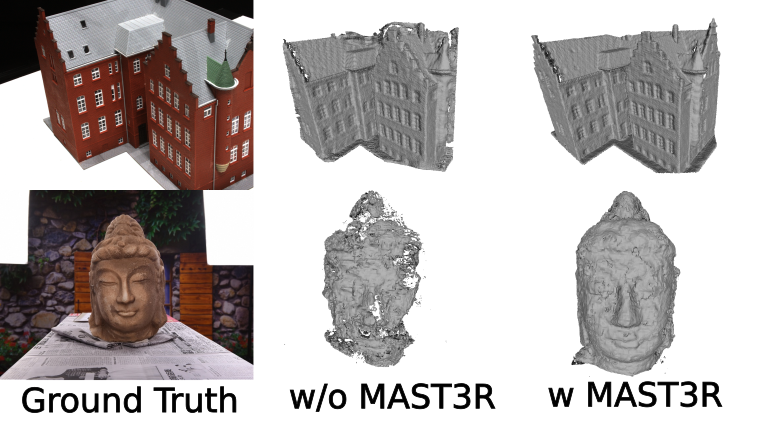
\includegraphics[width=1.0\linewidth]{figs/Ablation.png}
%     % \vspace{-15pt}
%     \caption{Left: Groud Truth image, Middle: Without MASt3R features, Right : With MASt3R features}
%     \label{fig:ablation}
% \end{figure}

\subsection{Inference time}
Once we infer pixel-aligned 2DGS parameters in a feed-forward manner, we can leverage them to render our depth maps significantly faster than previous generalizable implicit methods for reconstruction. We provide here inference speeds for ours and main baselines VolRecon \cite{ren2023volrecon}, ReTR \cite{liang2024retr}, GeoTransfer \cite{jena2024geotransfer} and UfoRecon \cite{na2024uforecon}. Depth map inference times is about $30$s as reported in their respective supplementary sections, while for UfoRecon \cite{na2024uforecon} it is higher at around $60$s. We reproduced this on a RTX A$6000$ and we obtained $0.88$s for ours, against $32$s for GeoTransfer \cite{jena2024geotransfer}, $31$s for VolRecon \cite{ren2023volrecon}, $37$s for ReTR \cite{liang2024retr}, and $66$s for UfoRecon \cite{na2024uforecon}.


